\newpage

\subsection{Schnittstellenbeschreibung und Integration der Komponenten}

Damit eine Gesamtintegration geplant werden kann, wurden beim Entwurf des Systems Schnittstellen auf C-Ebene zwischen den Komponenten festgelegt.

Folgendes Diagramm zeigt die Relation und Interaktion der 4 Komponenten miteinander:


\begin{figure}[H]
   	\centering
   	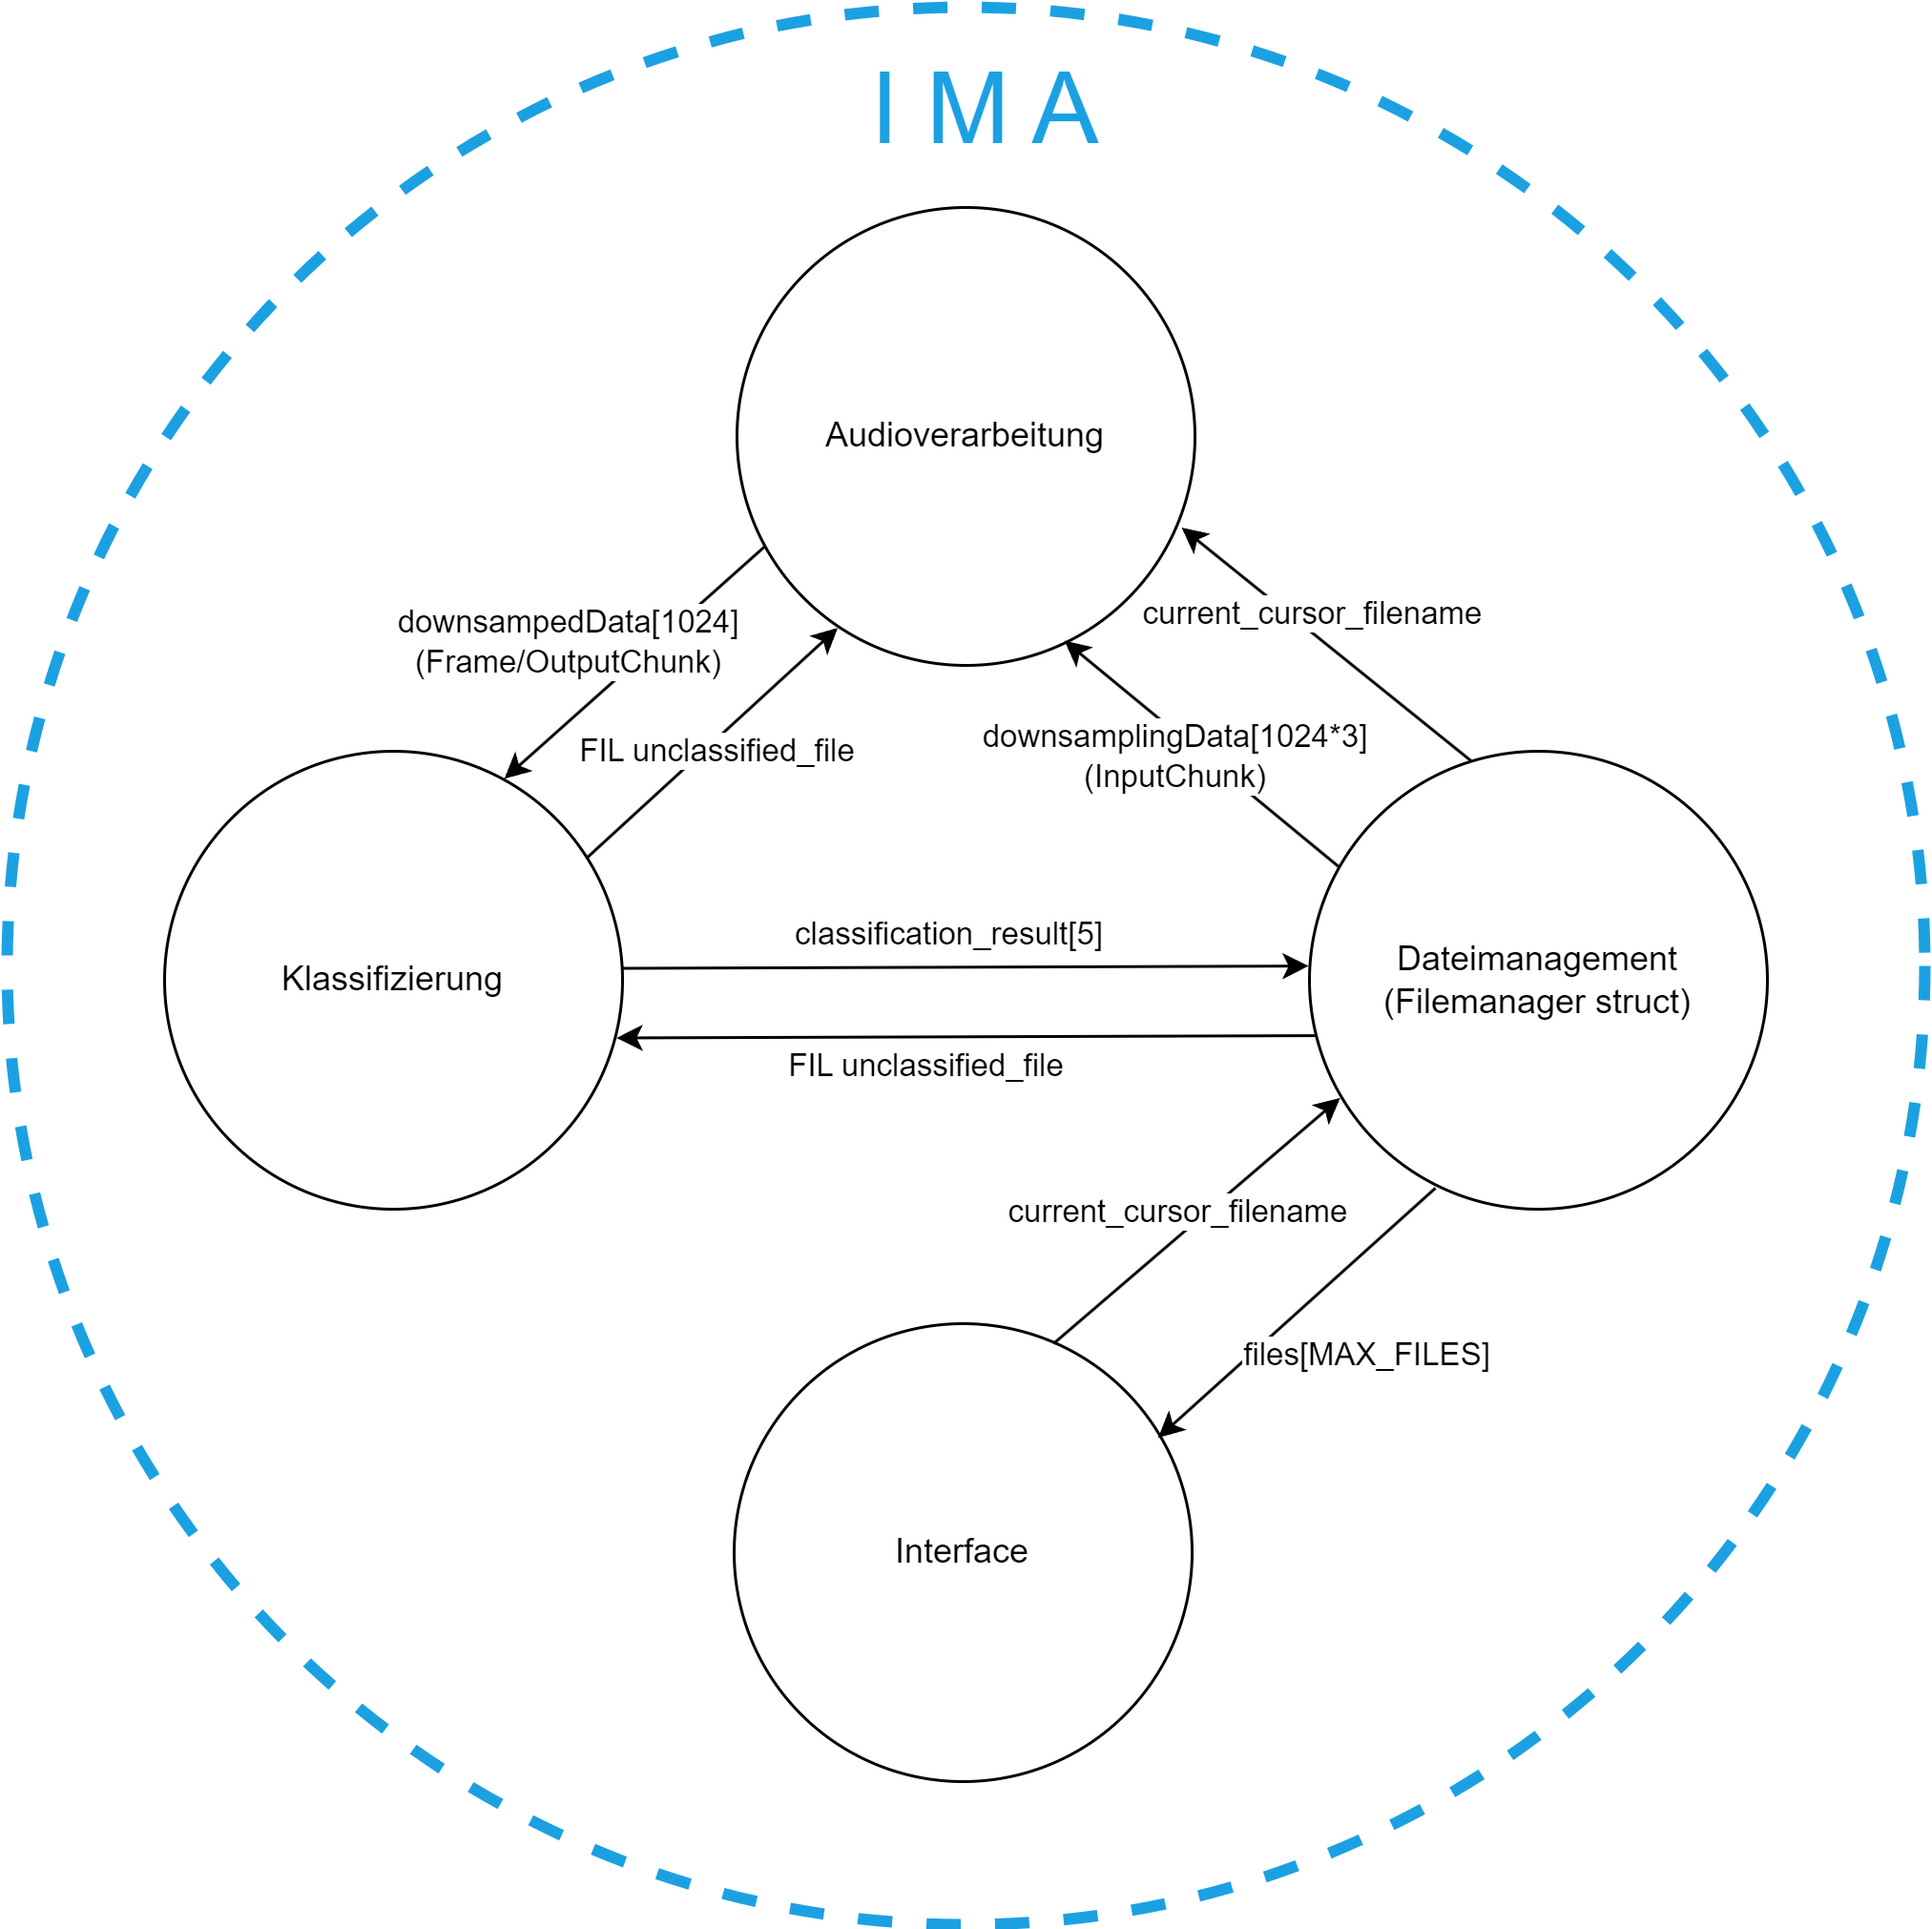
\includegraphics[width=0.8\textwidth]{images/04_spezifikation/komponentendiagramm.drawio.png}
   	\caption{Komponentendiagramm}
   	\label{fig:komponentendiagramm}
\end{figure}

Das \textbf{Dateimanagement} ist der zentrale Knotenpunkt des Gesamtsystems. Es dient zunächst als Zugriffspunkt auf die Samples anhand ihrer Namen. 

\subsubsection{Interaktion Downsampling} 

Bevor die Klassifizierung durchgeführt wird, müssen die zu klassifizierenden Audiodaten von der \textbf{Audioverarbeitungs}-Komponente in das richtige Format gebracht werden.
Die \textbf{Klassifizierung} übergibt den FATFS-Filehandle des herunterzusamplenden Files \mintinline{c}|FIL unclassified_file|. Mit dem Filehandle greift Die \textbf{Audioverarbeitung} auf die Datei zu und liest sich Chunkweise die \mintinline{c}|downsamplingData[1024*3]|. Die heruntergesampleten Daten \mintinline{c}|downsampledData[1024]| werden dann an die \textbf{Klassifizierung} zurück gegeben.

\subsubsection{Interaktion Klassifizierung} 

Die für das Spektrogramm benötigten heruntergesampelten Daten werden zur \textbf{Klassifizierung} weitergeleitet. Basierend auf dem Spektrogramm werden die Dateien anhand ihrer Klangmerkmale klassifiziert. Die Ergebnisse dieser Klassifikation werden in \mintinline{c}|classification_result[5]| gespeichert. Dieses Array wird anschließend an das Dateimanagement übergeben und wird dem Sample zugeordent.

\subsubsection{Interaktion Interfacing}
 
Das Interface ruft alle Dateien aus dem \mintinline{c}|FileManager Struct| in \mintinline{c}|files[MAX_FILES]| ab. Es filtert die Dateien basierend auf den festgelegten Filtereinstellungen und speichert die übereinstimmenden Dateien in \mintinline{c}|shownFiles[MAX_FILES]|.

Beim Auswählen eines Samples wird dessen Name in \mintinline{c}|current_cursor_filename| gespeichert welcher ein Part den \boldinline{FileManager} ist. Die \boldinline{Audioverarbeitung} greift auf diesen Namen zu, um das Sample zu laden und abzuspielen.

